\section{Sparsity and LASSO} \label{sec:prob4}
In this section, we used the sklearn Python implementation of the LASSO algorithm to model a dataset.

The raw x values are transformed into a feature vector with basis:
\begin{equation}
	\phi(x)=(x,sin(0.4\pi x \cdot 1), sin(0.4\pi x \cdot 2), ... , sin(0.4\pi x \cdot 12))
\end{equation}
The weights $w^T$ are used to map inputs $x$ to outputs $y$ through the basis $\phi(x)$, according to $y = w^T \phi(x)$. The dataset was generated using a true weight $w^T_{true}$ with small noise $\epsilon$, as $y = w^T_{true} \phi(x) + \epsilon$.


\begin{figure}
	\centering
	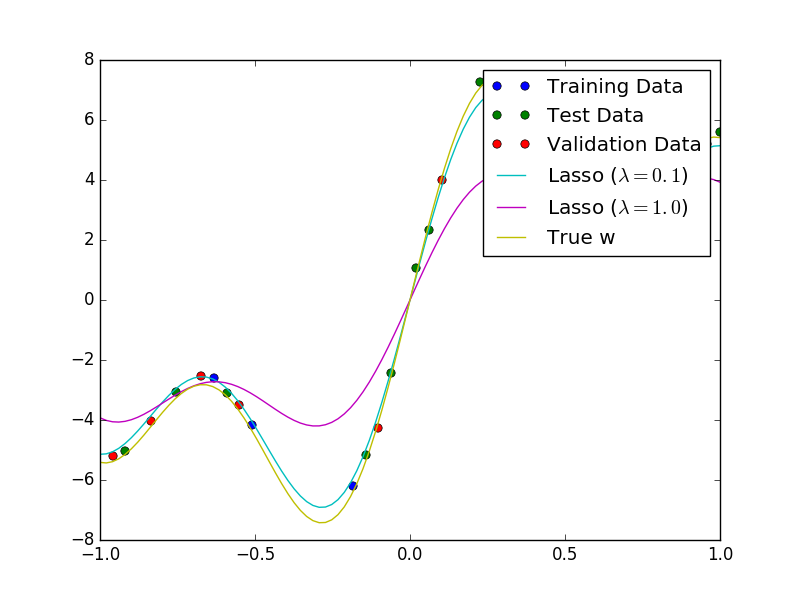
\includegraphics [trim=0 0 0 0, clip, angle=0, width=0.8\columnwidth,
	keepaspectratio]{figures/4_methods}
	\caption{The test, training, and validation data points are plotted along with models using true w values, LASSO's learned w values for two different regularization levels.} 
	\label{fig:4_methods} 
\end{figure}

\begin{figure}
	\centering
	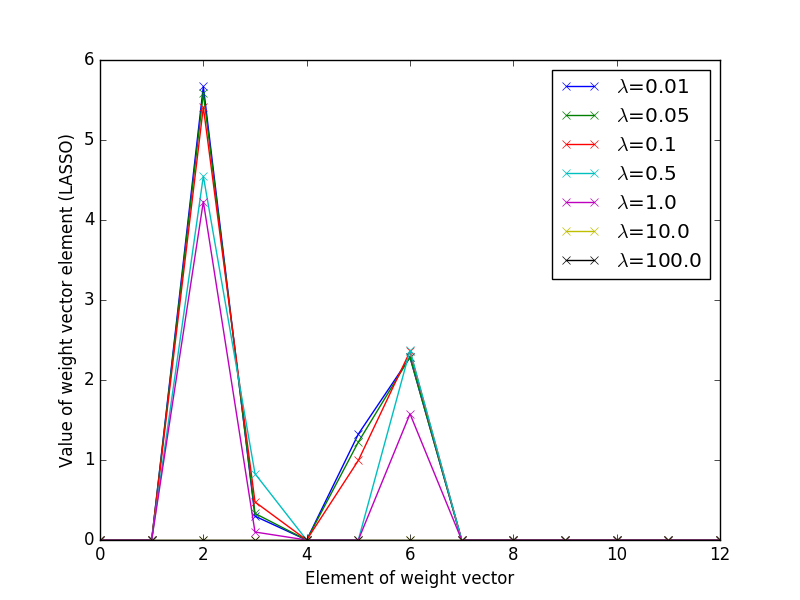
\includegraphics [trim=0 0 0 0, clip, angle=0, width=0.8\columnwidth,
	keepaspectratio]{figures/4_lasso_lambda}
	\caption{LASSO's learned weights are shown for several $\lambda$ values. When $\lambda$ is small, more of the weight terms are non-zero because regularization has little effect on the cost function.} 
	\label{fig:4_lasso_lambda} 
\end{figure}

\begin{figure}
	\centering
	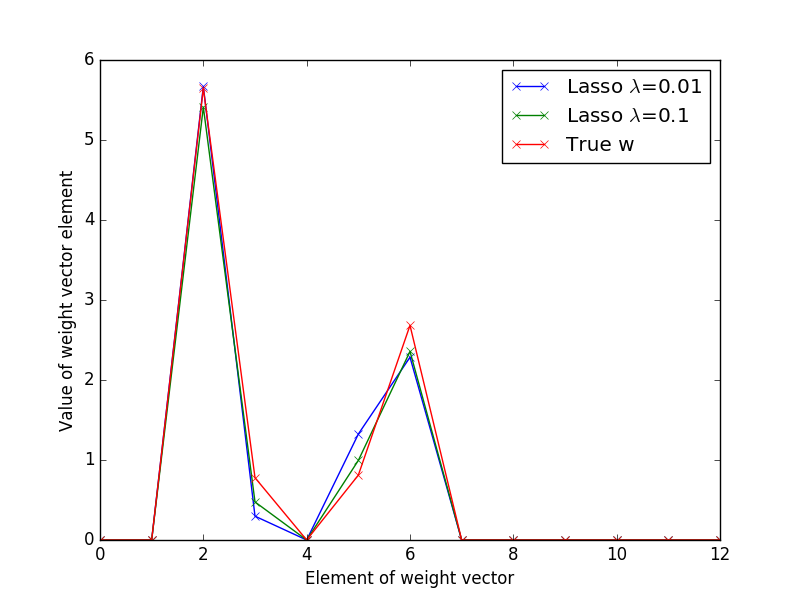
\includegraphics [trim=0 0 0 0, clip, angle=0, width=0.8\columnwidth,
	keepaspectratio]{figures/4_compare_w}
	\caption{The learned weights of LASSO are compared with the true weights.} 
	\label{fig:4_compare_w} 
\end{figure}











